% 2026.01.28
% use XeLaTeX
%Contributor: Underdog——Yao Zhihui,Yang Zijie,Lin Chen



\documentclass[twoside, fontset=windows]{ctexart}
\usepackage{graphicx}
\usepackage{geometry}%设置页边距
\usepackage{fancyhdr}%设置页眉页脚
\usepackage[backend=biber, style=gb7714-2015]{biblatex}
\usepackage{xeCJK} 
\usepackage{setspace}

\addbibresource{references.bib} % 必须指定 .bib 文件（含扩展名）

%设置文章格式
\geometry{a4paper, left=2.5cm, right=2.5cm, top=4cm, bottom=2cm}
\pagestyle{fancy}
\fancyhf{}
\fancyhead[CO]{阳光学院本科生毕业论文（设计）}
\fancyhead[CE]{偶数页页眉（题目）}
\cfoot{\thepage}

\setCJKfamilyfont{hwxk}{华文行楷}
\newcommand*{\xk}{\CJKfamily{hwxk}}


\ctexset{
  % 一级标题：消除段后空白，避免与二级标题叠加
  section={
    format=\centering\heiti\zihao{-2},
    nameformat=\heiti\zihao{-2},
    afterskip=0pt,          % 
  },
  % 二级标题：保持原设置
  subsection={
    format=\heiti\zihao{-3},
    nameformat=\heiti\zihao{-3},
    beforeskip=1\baselineskip,  % 空一行
    afterskip=1\baselineskip    % 空一行,   
  },
  % 三级标题
  subsubsection={
    format=\heiti\zihao{-4}\setlength{\baselineskip}{20pt}\selectfont,
    indent=1em,
    beforeskip=0.5\baselineskip,
    afterskip=0.5\baselineskip,
  }
}

%封面
\title{\zihao{0}\xk{阳\hspace{0.5em}光\hspace{0.5em}学\hspace{0.5em}院}}
\author{作者}

\begin{document}
\maketitle
\newpage
\zihao{-4}
%综述
\thispagestyle{empty}
\begin{center}
  \heiti\zihao{-2}你的题目
  
  \vspace{1em}  
  \heiti\zihao{4}摘要
\end{center}

{\songti\zihao{-4}
机器人技术领域的研究一直以来都十分热门，最近几年机器人开始被广泛应用于各种各样的产业，并且机器人技术的研究和扩展的进度也越来越迅速。机器人的智能化技术开始走进人们的日常生活中，让机器人替代人们完成一些文字书写、绘画等任务，具有一定的实际应用意义。因此课题选择了写字机器人的设计与实现。

系统包含上下位机两个部分。上位机包含了PC控制端和手机APP端；下位机包含了Arduino UNO、A4988电机驱动模块、HC-06蓝牙模块、步进电机、金属小舵机以及CoreXY结构机械臂等组成。系统选择两个自由度，采用Arduino UNO作为控制器，在PC控制端上将图片转换成坐标形式的G代码,再通过串口把文件发送给下位机,下位机编程实现像素扫描算法、直线插补算法和圆弧形插补算法,输出PWM脉冲和电平控制步进电机和舵机前进或者后退来完成写字。步进电机由A4988电机驱动设备来驱动，每发来一个PWM脉冲就前进或者后退一步，实现了对距离的精确控制。课题还设计了一个手机端APP，手机端连接好蓝牙后，在手机APP的文件导入界面导入转换好的G代码文件，再设置好写字起点后即可开始写字。课题上位机手机端APP是以Android Studio开发软件进行开发的，手机端APP的功能模块以及UI界面设计是采用Java语言来编程实现的。

经过实验测试，系统的功能基本全部实现，能够完成各种字体的文字书写、绘画等功能，还可以通过手机端APP对下位机进行远程控制。系统书写文字和绘制图形的效果较好，字体的精确度和精美度较好。

}
\vspace{1em}
{\heiti \zihao{-4}\raggedleft 关键词：xx\hspace{2em} xx\hspace{2em} xx}

\newpage
\tableofcontents
\thispagestyle{empty}
\newpage

\section{绪论}
  \subsection{课题研究背景和意义}
  {\zihao{-4}
  人工智能作为一门当今人们最为常用的技术科学之一，越来越多地被运用到各个领域。人工智能可以对人的意识、思维的信息过程进行模拟，虽然无法做到真正的人工智能，但在科技的进步中尽量做到能够像人那样思考，从而实现向人类智慧靠近，做到真正的智能。人工智能是在了解了智能的本质并根据人类的智慧作出反应之后，产生一种与人类相似的智能机器，这种技术即为人工智能。人工智能从诞生以来，理论和技术日益成熟，}在现代科技的发展过程中，它的应用领域还在不断扩大。想象在不久的将来，人们的生活会因人工智能产生极大的变化。
  \subsection{课题研究现状}
  近年来，随着机器人技术的不断发展，写字机器人作为一种新兴的智能设备
  \subsection{研究思路与研究内容}
  该设计思路是采用了Arduino UNO作为系统核心控制器，写字臂的结构上参照了激光雕刻机的CoreXY结构，因为相对其他结构来说CoreXY结构写字会更加稳定一些。

  系统研究内容上分为下位机和上位机两部分。
  下位机部分先完成硬件部分。采用Arduino UNO作为系统核心控制器，选用稳定结构的机械臂组装一个能平稳放置在台面上的机器人，写字臂可以插入圆珠笔或画笔。接着研究控制写字臂的写字算法，完成软件编程。能够实现书写文字的任务，能与手机端进行信息的收发，来对机器人进行控制，使其能够完成指定文字的书写或者图片的绘画。最后是通信模块的选择，选用了HC-06蓝牙通信模块，用于手机端和机器人之间的通信，保证信息的准确交互。

  上位机部分主要完成一个手机APP应用程序开发。选用了Android Studio开发平台和Java开发语言，设计出一个简易的交互界面，用来远程控制机器人，以及实时接收监控信息。

  \subsection{论文结构}
  本文内容具体分成以下五个章节。
第一章：绪论。这章介绍写字机器人的研究背景、意义、当前机器人的研究现状和本课题机器人的研究思路和研究内容。 

第二章：系统方案设计。先介绍了系统总体设计，然后介绍了系统开发技术。 

第三章：系统硬件设计。主要介绍硬件电路设计、原理图和各个模块。

第四章：系统软件设计。主要介绍了软件实现的流程图和两个算法的流程。

第五章：系统测试。介绍最终的测试情况，包括结果和分析。

最后是结论，对本课题已实现的功能和制作过程中解决的问题，还有今后如何改进和完善。 
\newpage

\section{系统方案设计}
  \subsection{系统总体设计}
  本课题整体系统由电脑端、手机移动端、Arduino UNO控制器、电机驱动设备、舵机和电机6部分组成。电脑端和手机移动端是上位机控制器，下位机控制器由Arduino UNO系统构成，电机和舵机是下位机的执行器[3]。上位机电脑端将想让机器人写的内容经过Inkscape图片转换软件转换成文件后缀为.nc或.gcode的文件。然后电脑端通过串口将文件发给下位机，手机APP端通过蓝牙发给下位机，使写字机器人执行文件中的坐标信息。下位机中Arduino UNO系统通过串口或者蓝牙接收上位机或手机APP发送过来的文件，将发送过来的文件识别并转换，再由下位机控制器中控制电机和舵机的程序控制电机和舵机完成写字的动作。写字机器人总框图如图1所示。
  \begin{figure}[h]
    \centering
    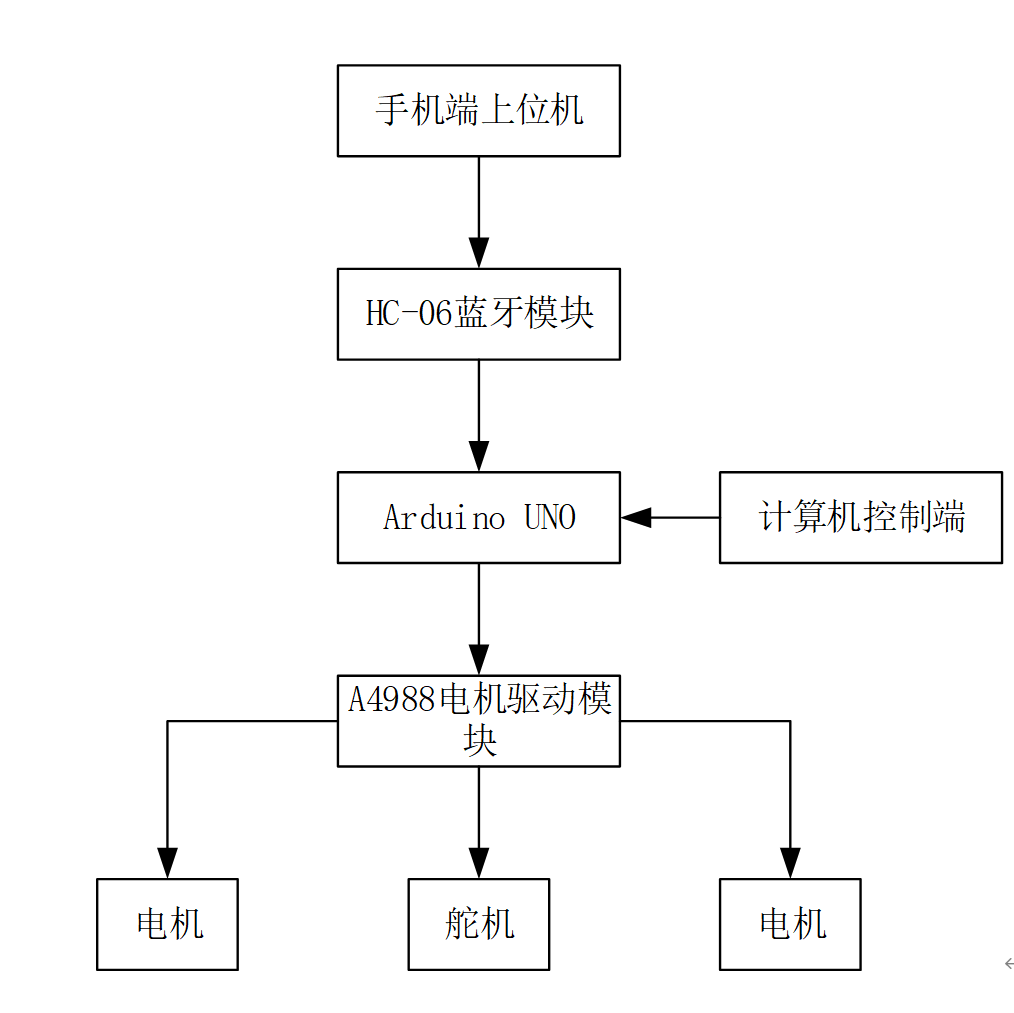
\includegraphics[width=0.8\textwidth]{figure/8f43da56-7d4d-4671-bd29-e7535ec9ea50.png}
    \caption{写字机器人系统框图}
  \end{figure}
  \subsection{系统开发技术}
  本课题的上位机APP软件是以Android Studio开发工具进行开发,主要通过Java语言来进行APP的蓝牙功能实现的编写,以及简单UI界面的设计,达到点击UI界面的按钮来进行发送指定数据控制写字机器人写字的功能。下位机系统核心控制器Arduino UNO主要使用Arduino IDE开发。

  Arduino IDE是为开发Arduino而设计的，专门用于Arduino程序的开发，具有开放源代码的原理图设计，ISP支持在线刻录，同时兼容C、Processing等多种程序。
    \subsubsection{系统框架}
    Android系统体系结构图如图2-3所示。Android系统四层架构分别是:
    （1）Linux内核层

    这一层是软件和硬件的抽象层，它的系统核心服务也是以此为基础的,Linux内核层也为各类设备的驱动提供了服务[4]。

    （2）系统运行库层

    这一层是应用程序支撑的框架，由特定的库来提供支持。这层还有Android运行库,包括核心库和虚拟机,核心库提供了调用所需的函数,还有一些核心API[5]。

    （3）应用框架层

    这一层是为构建应用程序提供服务，Android中的部分核心应用即为通过这些API完成。

    （4）应用程序层

    手机上的所有应用程序都是属于应用层,就如手机的浏览器、下载的游戏等,本课题中作为上位机的APP也是属于这个层。
    \newpage

\section{系统硬件设计}
  \subsection{XXXX结构设计}
  整体的框架用的8mm光轴和铝合金支架作为骨架，采用的是CoreXY结构，整体结构相较其他结构也比较紧凑，减少了运动部件的重量，可以适当提高电机的加速度。如图3-1所示。
  \subsection{Arduino UNO系统}
  本课题的Arduino UNO系统作为下位机核心控制器[6]，下位机通过串口或者蓝牙接收上位机发来已转换成坐标形式的G代码文件，再通过内部写字算法程序转换，输出控制脉冲和方向电平控制步进电机运作和舵机的抬笔和落笔\cite{TXXB20260123004}。
  \subsection{A4988电机驱动模块}
  \subsection{42步进电机}
  \subsection{舵机模块}
  \subsection{蓝牙模块}
\section{系统软件设计}
  \subsection{系统软件开发环境}
  \subsection{下位机设计-写字机械臂端}
  \subsection{像素扫描算法}
  \subsection{直线插补算法}


\nocite{*}
\printbibliography[title=参考文献, heading=bibintoc]

\end{document}